\section{Method}
\label{sec:method}
\begin{figure}[t]
  \centering
  \vspace*{2mm}
  \subfloat[]{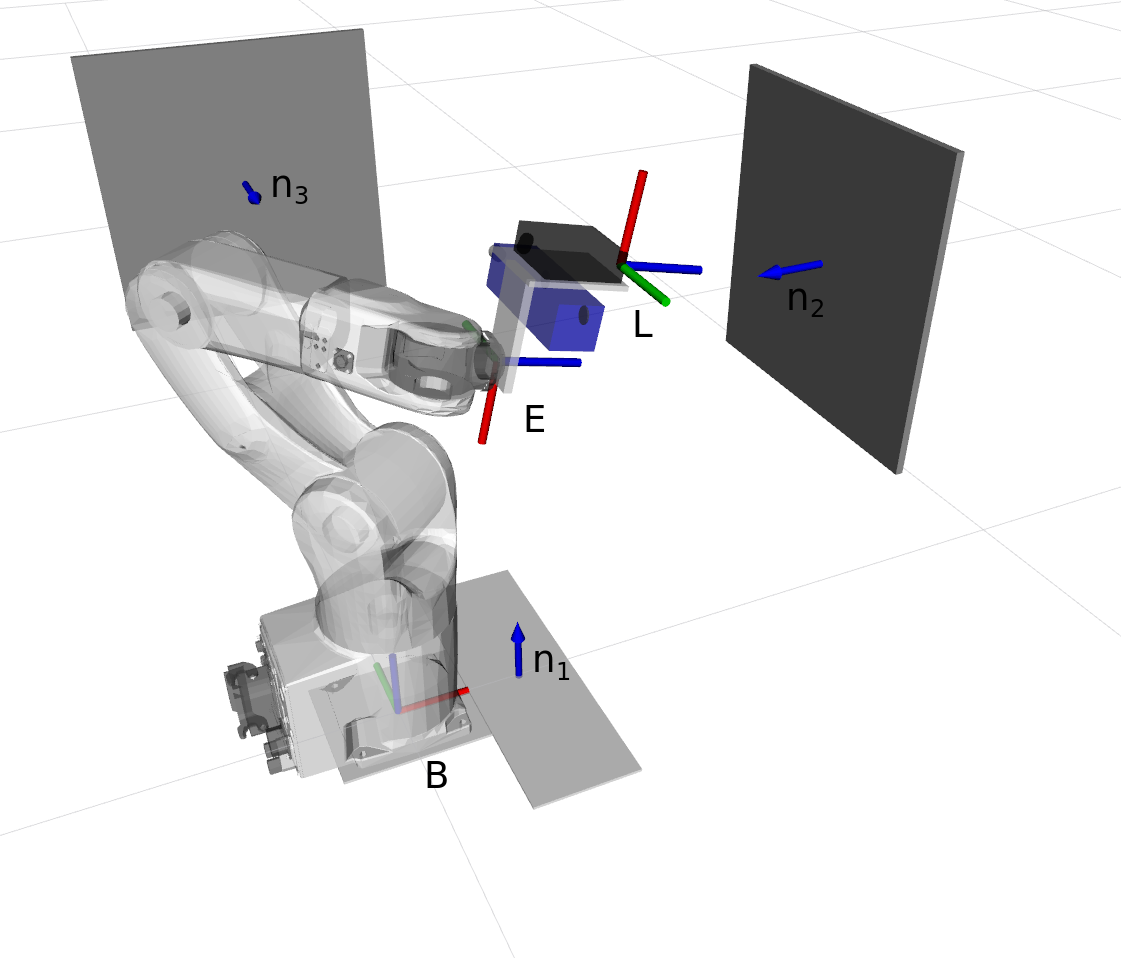
\includegraphics[height=60mm]{robot_setup}}
  \caption{Robot setup for the calibration}
  \label{fig:robot_setup}
\end{figure}


\renewcommand{\arraystretch}{1.5}
\begin{table}[htp]
\caption{Robot DH Parameters}
\label{tab:dh_params}
\centering
\begin{tabular}{c c c c c}
\toprule
i &  \textbf{$\alpha_i \;[^o]$} & \textbf{$a_i \;[mm]$} &  \textbf{$\theta_i \;[^o]$}  & \textbf{$d_i \;[mm]$}\\
\midrule
1 & 0.0 & 0.0 & 0.0 & 345.0\\
2 & -90.0 & 0.0 & -90.0 & 0.0\\
3 & 0.0 & 305.0 & 90.0 & 0.0\\
4 & 90.0 & -10.0 & 0.0 & 300.0\\
5 & -90.0 & 0.0 & 0.0 & 0.0\\
6 & 90.0 & 0.0 & 0.0 & 70.0\\
\bottomrule
\end{tabular}
\end{table}

The calibration setup is depicted in \fref{fig:robot_setup}, where three roughly perpendicular planes ($k=1,2,3$) are placed around the robot. An \ac{lrf} is attached to the robot flange. For each plane, the robot is moved to $N$ poses such that the \ac{lrf}'s ray is directed to the respective plane. One data set from the \ac{lrf} consists of hundreds of data points, so $M$ data points are selected from the \ac{lrf} data for each pose, and the robot's joint angles are recorded. 

This section provides the detail on how to calibrate both the extrinsic parameters of the LRF and the robot's kinematic parameters. First, the initial estimate of the LRF extrinsic parameter is obtained by using the linear least squares method based on the data from one of the planes. After that, the LRF extrinsic parameters and the robot's kinematic parameters are optimized simultaneously to satisfy the three planar constraints using Levenberg-Marquardt nonlinear optimization method. Finally, we explain how \ac{svd} can be used to analyse which calibration parameters are identifiable, and the steps to handle the unidentifiable parameters are then presented. 
\subsection{Initial Estimate of the \ac{lrf} Extrinsic Parameters}
\label{sec:first_step}
To obtain an initial estimate of the \ac{lrf} extrinsic parameters, only the data from one plane is necessary. Arbitrarily, the bottom plane $plane 1$ is chosen. The extrinsic parameters of the \ac{lrf} ${^E}\vb*{T}_L$, i.e. the homogeneous transformation from the robot flange coordinate frame to the \ac{lrf} coordinate frame, is estimated by the following calculation. 

Let the subscript/superscript $B$, $E$, and $L$ denote the coordinate frame of the robot base, the robot flange, and the \ac{lrf}, while the subscript $i$, $j$, and $k$ refer to the \ac{lrf} data point index, the robot pose index, and the plane index respectively. Let $\vb*{p}_{ji}$ be one of the data points from the \ac{lrf} which lies on the $plane 1$, $\vb*{n}_1$ be the normal unit vector of $plane 1$, and $l_1$ be the perpendicular distance from the origin of the robot coordinate system to $plane 1$.  Since $\vb*{p}_{ji}$ is located on the $plane 1$, it has to satisfy the following constraint, 
  \begin{equation}
  \label{eq:1}
  {^B}\vb*{n}_1 ^T \cdot\; {^B}\vb*{p}_{ji}  - {^B}l_1 = 0 \; .
   \end{equation}
${^B}\vb*{p}_{ji}$ depends on the robot pose ${^B}\vb*{T}_{E,j}$ at pose index j and the \ac{lrf} extrinsic parameter ${^E}\vb*{T}_L$, so \eqref{eq:1}  can be expanded,
  \begin{equation}
  {{^B}\vb*{n}_1 ^{T}} \cdot\; {^B}\vb*{T}_{E,j} \cdot \; {^E}\vb*{T}_L \cdot \; {^L}\vb*{p}_{ji}  - {^B}l_1 = 0 \; .
  \end{equation}
${^B}\vb*{n}_1$ and $^{B}l_1$ are known approximately ($[0 \; 0\; 1\;0]$ and $0.0$), ${^B}\vb*{T}_{E,j}$ can be computed from the robot's joint angles at pose index $j$, and ${^L}\vb*{p}_{ji}$ is obtained from the laser. Let 
\begin{equation}
{\vb*{n}_j^{'}}^{T} = {^B}\vb*{n}_1 ^T \cdot {^B}\vb*{T}_{E,j} = 
\left[n^{'}_{j,1} \quad n^{'}_{j,2} \quad n^{'}_{j,3}  \quad n^{'}_{j,4} \right] \; , 
\end{equation}
then  
  \begin{equation}
  \label{eq:3}
  {\vb*{n}_j^{'}} ^T \cdot {^E}\vb*{T}_L \cdot {^L}\vb*{p}_{ji} - {^B}l_1 = 0 \; .
  \end{equation}
The only unknown in \eqref{eq:3} is ${^E}\vb*{T}_L$ which has 12 elements $r_{uv}$, where u and v denote the column and the row index of the matrix. Note that the fourth row of ${^E}\vb*{T}_L$ only consists of 0 and 1. 
Without any loss of generality, let's assume that the data points from the \ac{lrf} lie on the XZ planes of the laser frame $L$, so ${^L}\vb*{p}_{ji} = \left[{^L}p_{i,x} \quad 0 \quad {^L}p_{i,z}\quad 1\right]$. If we expand \eqref{eq:3} and rearrange such that the components of ${^E}\vb*{T}_L$ are stacked together as a vector $\vb*{\Phi}_L$, we have
\begin{equation}
\label{eq:4}
  {\vb*{x}_{ji}}^T \cdot \vb*{\Phi}_L = {^B}l_1 -  n^{'}_{j,4} \; , 
\end{equation}
where 
\begin{multline}
  \vb*{x}_{ji} = \left[{^L}p_{i,x}\;n^{'}_{j,1} \quad {^L}p_{i,x}\;n^{'}_{j,2}\quad {^L}p_{i,x}\;n^{'}_{j,3}\quad  {^L}p_{i,z}\;n^{'}_{j,1}\right. \\ 
\left. {^L}p_{i,z}\;n^{'}_{j,2}\quad {^L}p_{i,z}\;n^{'}_{j,3} \quad n^{'}_{j,1} \quad n^{'}_{j,2} \quad n^{'}_{j,3} \right]^T \; , 
\end{multline}
and
\begin{multline}
  \vb*{\Phi}_L= \left[r_{11} \quad r_{21} \quad r_{31} \quad r_{13} \quad r_{23} \quad r_{33} \quad r_{14} \quad r_{24}  \quad r_{34} \right] ^T \; .
\end{multline}
For each data point $i$, we obtain such equation as in \eqref{eq:4}. With $M$ data points per pose and a total of $N$ robot poses, there are $NM$ such equations. The equations can be stacked together to form the following matrix equation,
\begin{equation}
\label{eq:7}
  \vb*{X}   \vb*{\Phi}_L= \vb*{D} \; ,
\end{equation}
where 
\begin{equation}
\vb*{X} =\begin{bmatrix}
{\vb*{x}_{11}} \; \cdots \;{\vb*{x}_{1M}}\quad  {\vb*{x}_{21}} \; \cdots \; {\vb*{x}_{2M}}\;  \cdots \; {\vb*{x}_{NM}} 
\end{bmatrix}^T 
\end{equation}
and 
\begin{multline}
\vb*{D} =\left[
{^B}l_1 -  n^{'}_{1,4} \quad
\cdots \quad
{^B}l_1 -  n^{'}_{1,4} \quad
{^B}l_1 -  n^{'}_{2,4} \quad
\cdots  \quad
\right. \\
\left.
{^B}l_1 -  n^{'}_{2,4} \quad
\cdots \quad
{^B}l_1 -  n^{'}_{N,4} \quad  
\right]^T \quad .
\end{multline}
Equation \eqref{eq:7} can be solved by a linear least-square procedure to obtain $\vb*{\Phi}_L$. ${^E}\vb*{T}_L$ can then be computed from $\vb*{\Phi}_L$ as follows:
\begin{enumerate}
\item The parameters $[r_{11} \quad r_{21} \quad r_{31}]^T$ and $[r_{13} \quad r_{23} \quad r_{33}]^T$ are required to be unit vectors, so they have to be normalized. They consistute the first and the third column of the matrix ${^E}T_L$.
\item The parameters $[r_{14} \quad r_{24} \quad r_{34}]^T$ constitute the position component of the matrix ${^E}T_L$ (the 4\textit{th} column).
\item The parameters $[r_{12} \quad r_{22} \quad r_{32}]^T$ can be calculated as the cross product of  $[r_{13} \quad r_{23} \quad r_{33}]^T$ and $[r_{11} \quad r_{21} \quad r_{31}]^T$ .
\end{enumerate}

${^E}\vb*{T}_L$ has 12 parameters, but only 6 parameters are independent. To reduce the redundancy in the subsequent steps, the rotation part of ${^E}\vb*{T}_L$ is represented by the axis-angle representation $[r_x \quad r_y \quad r_z \quad r_{\theta}]$, while the position part is represented by  $[p_x \quad p_y\quad p_z]$.


\subsection{Optimizing both the \ac{lrf} Extrinsic Parameters and Robot's Kinematic Parameters}
\label{sec:second_step}
In the second step, the data from all the three planes are used to optimize the extrinsic parameters of the \ac{lrf}, the robot's kinematic parameters and the plane parameters. The objective function is described as follows:

\begin{equation}
 f (\vb*{\Phi}) =  \sum_{k=1}^{3} \sum_{j=1}^{N} \sum_{i=1}^{M} ({{^B}\vb*{n}_1}^T \cdot {^B}\vb*{p}_{ji} - {^B}l_k)^2
\end{equation}

The parameters $\vb*{\Phi}$ consist of the following:
\begin{enumerate}
\item Robot's kinematic parameters. We use the modified \textbf{DH} parameters \cite{Hayati1985} $[a_i \;, \alpha_i \;,\theta_i \;,d_i], i=1, 2, \cdots ,6$ to represent the robot's kinematics, so there are 24 \textbf{DH} parameters for a 6-\ac{dof} robot arm. 
\item \ac{lrf}'s extrinsic parameters. As mentioned in the previous section, we use the axis angle representation for the rotation part $[r_x \quad r_y \quad r_z \quad r_{\theta}]$, and $[p_x \quad p_y\quad p_z]$ for the position part. 
\item Plane parameters. Each plane can be described by a unit vector $[{^B}n_{k,x}\quad {^B}n_{k,y}\quad {^B}n_{k,z}]$ normal to the plane and its perpendicular distance from the robot base's coordinate system origin ${^B}l_{k}$, so there are 12 parameters for 3 planes.
\end{enumerate}

In total, there are 43 parameters to be optimized by minimizing the objective function $f(\vb*{\Phi})$. To do that, the number of data points $3NM$ have to exceed the number of parameters. The optimization problem is then solved using a Levenberg-Marquardt nonlinear optimizer \cite{Newville2014}. The objective function $f(\vb*{\Phi})$ uses the geometric constraints that all data points from the \ac{lrf} have to fall on the respective plane. Zhuang et al. \cite{Zhuang1999} prove that a calibration process with such constraints is equivalent to the calibration of a robot using end-point measurement in unconstrained calibration. 

For the unit vector parameters ($[r_x \quad r_y \quad r_z ]$ and  $[{^B}n_{k,x} \quad {^B}n_{k,y} \quad {^B}n_{k,z}]$), the following constraints are added to the optimization solver:
\begin{equation}
\label{eq:10}
{r_z} = \sqrt{1 - {r_x}^2 - {r_y}^2}
\end{equation}
\begin{equation}
\label{eq:11}
{^B}n_{k,z} = \sqrt{1 - {{^B}n_{k,x}}^2 - {{^B}n_{k,y}}^2}
\end{equation}

Further analysis on the observability of the parameters will be presented in the next section. 

\subsection{The identifiability of the calibration parameters}
\label{sec:third_step}

Depending on the chosen robot calibration poses and the robot's kinematic model, some of the calibration parameters might not be observable due to the redundancy among the parameters. This is a critical problem in calibration, as it will result in some of the parameters assuming erratic values which gives us unstable calibration result. To prevent that, we have to first analyse which calibration parameters are identifiable and which are not. 

Following the approach in \cite{Joubair2015} and \cite{Hollerbach1996}, SVD is applied on the identification Jacobian matrix $\vb*{J}$. $\vb*{J}$ can be computed as follows. Let  $f_{kji}(\Phi)$ be the constraint equation on the data point $i$ at the robot pose $j$ and on the plane k, 
\begin{equation}
\label{eq:12}
 f_{kji}(\vb*{\Phi}) =  {{^B}\vb*{n}_k}^T \cdot {^B}\vb*{p}_{ji} - {^B}l_k \; .
\end{equation}
Then $\vb*{J}$ can be computed by differentiating \eqref{eq:12} for all the data points $i = 1, \cdots, M$ at robot poses $j = 1, \cdots, N$ and for all the planes $k=1,2,3$, and stack them together as a matrix,
\renewcommand\arraystretch{1.5}
\begin{equation}
\vb*{J} = \begin{bmatrix}
 \frac{\partial f_{111}(\vb*{\Phi})}{\partial\vb*{\Phi}} \quad
 \frac{\partial f_{112}(\vb*{\Phi})}{\partial\vb*{\Phi}} \quad
 \cdots  \quad
 \frac{\partial f_{3MN}(\vb*{\Phi})}{\partial\vb*{\Phi}} \quad
	\end{bmatrix} ^T \; .
\end{equation}

We can then apply SVD to the matrix $\vb*{J}$,
\begin{equation}
 \vb*{J} = \vb*{U}\vb*{\Sigma}\vb*{V}^T \; .
\end{equation}
Note that for this identification step, the parameters $[r_z \quad {^B}n_{1,z}\quad {^B}n_{2,z}\quad {^B}n_{3,z}]$ are excluded from the parameters vector $\Phi$, since those four parameters are obtained as linear combinations of other parameters (Equation \eqref{eq:10} and \eqref{eq:11}). That leaves us with 43-4 = 39 parameters in $\vb*{\Phi}$, which correlates to the 39 singular numbers in $\Sigma$. The number of zero-value singular numbers in $\Sigma$ is then equal to the number of unidentifiable parameters in the calibration procedure. For a given zero-value singular number $\sigma_r$, the r\textit{th} column vector of the matrix $\vb*{V}$ is the linear combination of the parameters $\vb*{\Phi}$ which cannot be identified independently. 

In this paper, we use a Denso VS060 6-\ac{dof} industrial manipulator with its \textbf{DH} parameters presented in \tref{tab:dh_params}. The \ac{lrf}'s frame is defined such that the rotation part $[r_x \quad r_y \quad r_z \quad r_{\theta}] = [0 \quad 0 \quad 1 \quad \pi]$, and the position part $[p_x \quad p_y\quad p_z] = [-0.1275 \quad -0.033 \quad 0.1015]$. Applying the identifiability analysis to the system, we found that there are 7 redundant parameters out of the 39 parameters. By analysing the matrix $\vb*{V}$, these redundant parameters are due to:
\begin{enumerate}
\item The parameters $d_6$ (the translation along the z-axis of the 6\textit{th} link frame on the flange) and $p_z$ (the z coordinate of the \ac{lrf} frame) are redundant. Physically this means that if we shift the origin of the frame 6 in its z direction by changing $d_6$, we can compensate by shifting the origin of the \ac{lrf} frame in the opposite direction by changing $p_z$.
\item The parameters $\theta_6$ and $r_\theta$ are redundant. These are the rotation of the robot's last link and the rotation of the \ac{lrf} frame around the same z-axis. 
\item The parameters $d_2$ and $d_3$ are redundant. These correspond to the shift in the z-axis direction of the 2\textit{nd} and 3\textit{rd} link frames respectively, which are along the same direction, so they will compensate each other. 
\item Lastly, we have four redundant parameters due to the linear combination of the first link's DH parameters $[a_1, \alpha_1, \theta_1, d_1 ]$ and the three calibration planes' parameters. Physically, this relates to the fact that we can adjust the location of the base frame freely by changing the value of $[a_1, \alpha_1, \theta_1, d_1]$, and the planes' parameters will adjust according to the new base location. In other words, the base coordinate is not constrained (floating). 
\end{enumerate}

Note that the same result will be obtained for other robots with similar kinematic structure as Denso VS060. 

For each pair of the redundant parameters, we can assign a fix value to one of the parameters. In this case, we set the value of the parameters [$d_6, \theta_6, d_2, a_1, \alpha_1, \theta_1, d_1$] to keep their initial model's values. 
